%TC:ignore
\documentclass{article}
\usepackage{caption}
\usepackage{xcolor, colortbl}
\definecolor{BLUELINK}{HTML}{0645AD}
\definecolor{DARKBLUELINK}{HTML}{0B0080}
\PassOptionsToPackage{hyphens}{url}
\usepackage[colorlinks=false]{hyperref}
% for linking between references, figures, TOC, etc in the pdf document
\hypersetup{colorlinks,
    linkcolor=DARKBLUELINK,
    anchorcolor=DARKBLUELINK,
    citecolor=DARKBLUELINK,
    filecolor=DARKBLUELINK,
    menucolor=DARKBLUELINK,
    urlcolor=BLUELINK
} % Color citation links in purple
\PassOptionsToPackage{unicode}{hyperref}
\PassOptionsToPackage{naturalnames}{hyperref}

\usepackage[backend=biber,eprint=false,isbn=false,url=false,intitle=true,style=nature,date=year]{biblatex}
\addbibresource{codon_models.bib}

\usepackage[margin=50pt]{geometry}
\usepackage{amssymb,amsfonts,amsmath,amsthm,mathtools}
\usepackage{lmodern}
\usepackage{bm,bbold}
\usepackage{verbatim}
\usepackage{float}
\usepackage{listings, enumerate, enumitem}
\usepackage[export]{adjustbox}
\usepackage{tabu}
\usepackage{longtable}
\tabulinesep=0.6mm
\newcommand\cellwidth{\TX@col@width}
\usepackage{hhline}
\setlength{\arrayrulewidth}{1.2pt}
\usepackage{multicol,multirow,array}
\usepackage{etoolbox}
\AtBeginEnvironment{tabu}{\footnotesize}
\usepackage{booktabs}
\usepackage{graphicx}
\pdfinclusioncopyfonts=1

\renewcommand{\thetable}{S\arabic{table}}
\renewcommand{\thefigure}{S\arabic{figure}}

\newcommand{\UniDimArray}[1]{\bm{#1}}
\newcommand{\BiDimArray}[1]{\bm{#1}}
\DeclareMathOperator{\E}{\mathbb{E}}
\DeclareMathOperator{\Var}{\textrm{Var}}
\newcommand{\der}{\textrm{d}}
\newcommand{\e}{\textrm{e}}
\newcommand{\avg}[1]{\left< #1 \right>} % for average
\newcommand{\Ne}{N_{\textrm{e}}}
\newcommand{\proba}{\mathbb{P}}
\newcommand{\pfix}{\proba_{\textrm{fix}}}
\newcommand{\dn}{d_N}
\newcommand{\ds}{d_S}
\newcommand{\dnds}{\dn / \ds}
\newcommand{\Sphy}{S_{0}}
\newcommand{\Sphyclass}{\mathcal{C}}
\newcommand{\SphyMean}{\overline{\Sphy}}
\newcommand{\divDel}{\Sphy^{\text{d}}}
\newcommand{\divWeak}{\Sphy^{\text{n}}}
\newcommand{\divAdv}{\Sphy^{\text{b}}}
\newcommand{\PdivDel}{\proba \left[ \divDel \right]}
\newcommand{\PdivWeak}{\proba \left[ \divWeak \right]}
\newcommand{\PdivAdv}{\proba \left[ \divAdv \right]}
\newcommand{\given}{\mid}
\newcommand{\Spop}{S}
\newcommand{\SpopMean}{\overline{\Spop}}
\newcommand{\polyDel}{\Spop^{\text{d}}}
\newcommand{\polyNeutral}{\Spop^{\text{n}}}
\newcommand{\polyAdv}{\Spop^{\text{b}}}
\newcommand{\PpolyDel}{\proba \left[ \polyDel \right]}
\newcommand{\PpolyNeutral}{\proba \left[ \polyNeutral \right]}
\newcommand{\PpolyAdv}{\proba \left[ \polyAdv \right]}

\title{\textbf{Empirical evidence for beneficial mutations that are not adaptive innovations in mammals}}

\author{
    \large
    \textbf{T. {Latrille}$^{1}$, J. {Joseph}$^{2}$, D.~A. {Hartasánchez}$^{1}$, N. {Salamin}$^{1}$}\\
    \scriptsize $^{1}$Department of Computational Biology, Université de Lausanne, Lausanne, Switzerland\\
    \scriptsize $^{2}$Université de Lyon, Université Lyon 1, CNRS, VetAgro Sup, Laboratoire de Biométrie et Biologie Evolutive, UMR5558, Villeurbanne, France \\
    \texttt{\href{mailto:thibault.latrille@ens-lyon.org}{thibault.latrille@ens-lyon.org}} \\
}


\date{}

\begin{document}
    \maketitle
    \part*{Supplementary materials}
    \tableofcontents
    \clearpage

    \section{Mutation-selection codon models}\label{sec:site-specific-mutation-selection-codon-models}
    In BayesCode (\url{https://github.com/ThibaultLatrille/bayescode}), mutation-selection codon models are obtained by running \textit{mutselomega} for 2000 points of MCMC with the options:
    \begin{scriptsize}
        \begin{verbatim}
 mutselomega ---omegashift 0.0 --ncat 30 -a my_alignment.phy -t my_tree.newick -u 2000 my_genename
        \end{verbatim}
    \end{scriptsize}
    The collection of site-specific fitness profiles ($\UniDimArray{F^{(i)}}, \forall i$) are then obtained by running \textit{readmutselomega}, reading 1000 points of MCMC (first 1000 are considered as burn-in) with the options:
    \begin{scriptsize}
        \begin{verbatim}
 readmutselomega --every 1 --until 2000 --burnin 1000 --ss my_genename
        \end{verbatim}
    \end{scriptsize}
    The gene-specific $4 \times 4$ nucleotide mutation rate matrix ($\UniDimArray{\mu}$) is also obtained by running \textit{readmutselomega}, reading 1000 points of MCMC (first 1000 are considered as burn-in) with the options:
    \begin{scriptsize}
        \begin{verbatim}
 readmutselomega --every 1 --until 2000 --burnin 1000 --nuc my_genename
        \end{verbatim}
    \end{scriptsize}

    \subsection{Summary tables}\label{subsec:summary-table-mutsel}

    \subsubsection{$\dnds$ and beneficial back-mutations}
    \begin{center}
        \captionof{table}{$\dnds$ of beneficial back-mutations.}
        \scriptsize
        \begin{longtable*}{|l|l|r|r|r|r|r|r|}
            \toprule
            Population &             Species & Tajima $\theta_{\pi}$  & $\mathbb{P}_{div}[ S_0^{b} ]$ & $\omega $ & $\omega ( S_0^{d} )$ & $\omega ( S_0^{n} )$ & $\omega ( S_0^{b} )$ \\
            \midrule
            \endfirsthead

            \toprule
            Population &             Species & Tajima $\theta_{\pi}$  & $\mathbb{P}_{div}[ S_0^{b} ]$ & $\omega $ & $\omega ( S_0^{d} )$ & $\omega ( S_0^{n} )$ & $\omega ( S_0^{b} )$ \\
            \midrule
            \endhead
            \midrule
            \multicolumn{8}{r}{{Continued on next page}} \\
            \midrule
            \endfoot

            \bottomrule
            \endlastfoot
            Equus c. &      Equus caballus &               $ 0.002$ &                      $ 0.118$ &  $ 0.147$ &             $ 0.075$ &             $ 0.823$ &             $ 1.203$ \\
            Iran &          Bos taurus &               $ 0.002$ &                      $ 0.123$ &  $ 0.131$ &             $ 0.074$ &             $ 0.627$ &             $ 1.206$ \\
            Uganda &          Bos taurus &               $ 0.005$ &                      $ 0.125$ &  $ 0.134$ &             $ 0.075$ &             $ 0.637$ &             $ 1.252$ \\
            Australia &        Capra hircus &               $ 0.003$ &                      $ 0.121$ &  $ 0.125$ &             $ 0.068$ &             $ 0.629$ &             $ 1.099$ \\
            France &        Capra hircus &               $ 0.004$ &                      $ 0.120$ &  $ 0.126$ &             $ 0.068$ &             $ 0.633$ &             $ 1.102$ \\
            Iran (C. aegagrus) &        Capra hircus &               $ 0.004$ &                      $ 0.120$ &  $ 0.125$ &             $ 0.068$ &             $ 0.630$ &             $ 1.100$ \\
            Iran &        Capra hircus &               $ 0.004$ &                      $ 0.121$ &  $ 0.125$ &             $ 0.067$ &             $ 0.630$ &             $ 1.108$ \\
            Italy &        Capra hircus &               $ 0.004$ &                      $ 0.120$ &  $ 0.126$ &             $ 0.068$ &             $ 0.634$ &             $ 1.102$ \\
            Morocco &        Capra hircus &               $ 0.004$ &                      $ 0.122$ &  $ 0.125$ &             $ 0.067$ &             $ 0.631$ &             $ 1.112$ \\
            Iran &          Ovis aries &               $ 0.007$ &                      $ 0.109$ &  $ 0.146$ &             $ 0.091$ &             $ 0.616$ &             $ 1.148$ \\
            Iran (O. orientalis) &          Ovis aries &               $ 0.009$ &                      $ 0.108$ &  $ 0.148$ &             $ 0.093$ &             $ 0.617$ &             $ 1.145$ \\
            Iran (O. vignei) &          Ovis aries &               $ 0.007$ &                      $ 0.109$ &  $ 0.146$ &             $ 0.091$ &             $ 0.617$ &             $ 1.134$ \\
            Various &          Ovis aries &               $ 0.008$ &                      $ 0.107$ &  $ 0.148$ &             $ 0.093$ &             $ 0.617$ &             $ 1.134$ \\
            Morocco &          Ovis aries &               $ 0.008$ &                      $ 0.108$ &  $ 0.148$ &             $ 0.093$ &             $ 0.619$ &             $ 1.149$ \\
            Barbados & Chlorocebus sabaeus &               $ 0.004$ &                      $ 0.122$ &  $ 0.133$ &             $ 0.071$ &             $ 0.696$ &             $ 1.397$ \\
            Central Afr. Rep. & Chlorocebus sabaeus &               $ 0.006$ &                      $ 0.124$ &  $ 0.134$ &             $ 0.071$ &             $ 0.701$ &             $ 1.431$ \\
            Ethiopia & Chlorocebus sabaeus &               $ 0.005$ &                      $ 0.124$ &  $ 0.134$ &             $ 0.071$ &             $ 0.699$ &             $ 1.422$ \\
            Gambia & Chlorocebus sabaeus &               $ 0.005$ &                      $ 0.123$ &  $ 0.134$ &             $ 0.071$ &             $ 0.703$ &             $ 1.411$ \\
            Kenya & Chlorocebus sabaeus &               $ 0.005$ &                      $ 0.123$ &  $ 0.134$ &             $ 0.071$ &             $ 0.699$ &             $ 1.419$ \\
            Nevis & Chlorocebus sabaeus &               $ 0.003$ &                      $ 0.123$ &  $ 0.133$ &             $ 0.071$ &             $ 0.699$ &             $ 1.407$ \\
            South Africa & Chlorocebus sabaeus &               $ 0.006$ &                      $ 0.125$ &  $ 0.134$ &             $ 0.070$ &             $ 0.704$ &             $ 1.447$ \\
            Saint Kitts & Chlorocebus sabaeus &               $ 0.004$ &                      $ 0.123$ &  $ 0.133$ &             $ 0.070$ &             $ 0.699$ &             $ 1.413$ \\
            Zambia & Chlorocebus sabaeus &               $ 0.006$ &                      $ 0.123$ &  $ 0.134$ &             $ 0.071$ &             $ 0.699$ &             $ 1.410$ \\
            African &        Homo sapiens &               $ 0.002$ &                      $ 0.099$ &  $ 0.192$ &             $ 0.118$ &             $ 0.865$ &             $ 1.609$ \\
            Admixed American &        Homo sapiens &               $ 0.002$ &                      $ 0.099$ &  $ 0.192$ &             $ 0.118$ &             $ 0.865$ &             $ 1.607$ \\
            East Asian &        Homo sapiens &               $ 0.002$ &                      $ 0.098$ &  $ 0.192$ &             $ 0.118$ &             $ 0.869$ &             $ 1.607$ \\
            European &        Homo sapiens &               $ 0.002$ &                      $ 0.098$ &  $ 0.192$ &             $ 0.118$ &             $ 0.865$ &             $ 1.598$ \\
            South Asian &        Homo sapiens &               $ 0.002$ &                      $ 0.099$ &  $ 0.192$ &             $ 0.118$ &             $ 0.867$ &             $ 1.610$ \\
        \end{longtable*}
    \end{center}
    \begin{itemize}
        \item Tajima $\theta$ is the synonymous diversity.
        \item $\mathbb{P}_{div}[\Sphy > 1]$ is the proportion of substitutions in the terminal branch observed with a selection coefficient at the phylogenetic scale larger than 1 ($\Sphy > 1$).
        \item $\dn(\Sphy > 1) / \ds$ is the ratio of non-synonymous over synonymous divergence (also called $\dnds$) estimated for the non-synonymous substitutions in the terminal branch with a selection coefficient larger than 1 ($\Sphy > 1$).
        \item $\dn(\Sphy > 1) / \ds$ is the ratio of non-synonymous over synonymous divergence (also called $\dnds$) estimated for the non-synonymous substitutions in the terminal branch with a selection coefficient larger than 1 ($\Sphy > 1$).
        \item $\dn(\Sphy > 1) / \ds$ is the ratio of non-synonymous over synonymous divergence (also called $\dnds$) estimated for the non-synonymous substitutions in the terminal branch with a selection coefficient larger than 1 ($\Sphy > 1$).
    \end{itemize}

    \newpage
    \begin{center}
        \captionof{table}{$\dnds$ over-estimation due to beneficial back-mutations.}
        \scriptsize
        \begin{longtable*}{|l|l|r|r|r|r|r|}
            \toprule
            Population & Species & Tajima $\theta_{\pi}$ & $\mathbb{P}_{div}[\Sphy > 0]$ & $\dnds $ & $\dn(\Sphy < 0) / \ds$ & R($\dnds $) \\
            \midrule
            \endhead
            \midrule
            \multicolumn{7}{r}{{Continued on next page}} \\
            \midrule
            \endfoot

            \bottomrule
            \endlastfoot
            Equus c. &      Equus caballus &               $ 0.002$ &                $ 0.307$ &        $ 0.182$ &              $ 0.133$ &           $  27.0$ \\
            Iran &          Bos taurus &               $ 0.005$ &                $ 0.298$ &        $ 0.164$ &              $ 0.122$ &           $  26.1$ \\
            Uganda &          Bos taurus &               $ 0.005$ &                $ 0.303$ &        $ 0.167$ &              $ 0.123$ &           $  26.6$ \\
            Australia &        Capra hircus &               $ 0.003$ &                $ 0.301$ &        $ 0.157$ &              $ 0.116$ &           $  26.4$ \\
            France &        Capra hircus &               $ 0.003$ &                $ 0.300$ &        $ 0.158$ &              $ 0.116$ &           $  26.3$ \\
            Iran (C. aegagrus) &        Capra hircus &               $ 0.003$ &                $ 0.300$ &        $ 0.158$ &              $ 0.116$ &           $  26.3$ \\
            Iran &        Capra hircus &               $ 0.004$ &                $ 0.303$ &        $ 0.157$ &              $ 0.115$ &           $  26.6$ \\
            Italy &        Capra hircus &               $ 0.003$ &                $ 0.300$ &        $ 0.158$ &              $ 0.116$ &           $  26.3$ \\
            Morocco &        Capra hircus &               $ 0.004$ &                $ 0.303$ &        $ 0.157$ &              $ 0.115$ &           $  26.6$ \\
            Iran &          Ovis aries &               $ 0.007$ &                $ 0.266$ &        $ 0.179$ &              $ 0.138$ &           $  22.7$ \\
            Iran (O. orientalis) &          Ovis aries &               $ 0.009$ &                $ 0.265$ &        $ 0.180$ &              $ 0.140$ &           $  22.6$ \\
            Iran (O. vignei) &          Ovis aries &               $ 0.007$ &                $ 0.268$ &        $ 0.178$ &              $ 0.137$ &           $  22.8$ \\
            Various &          Ovis aries &               $ 0.009$ &                $ 0.264$ &        $ 0.180$ &              $ 0.140$ &           $  22.5$ \\
            Morocco &          Ovis aries &               $ 0.007$ &                $ 0.265$ &        $ 0.180$ &              $ 0.140$ &           $  22.6$ \\
            Barbados & Chlorocebus sabaeus &               $ 0.004$ &                $ 0.303$ &        $ 0.172$ &              $ 0.126$ &           $  26.8$ \\
            Central Afr. Rep. & Chlorocebus sabaeus &               $ 0.006$ &                $ 0.304$ &        $ 0.173$ &              $ 0.126$ &           $  27.0$ \\
            Ethiopia & Chlorocebus sabaeus &               $ 0.005$ &                $ 0.305$ &        $ 0.172$ &              $ 0.126$ &           $  27.1$ \\
            Gambia & Chlorocebus sabaeus &               $ 0.005$ &                $ 0.304$ &        $ 0.172$ &              $ 0.126$ &           $  26.9$ \\
            Kenya & Chlorocebus sabaeus &               $ 0.005$ &                $ 0.304$ &        $ 0.173$ &              $ 0.126$ &           $  27.0$ \\
            Nevis & Chlorocebus sabaeus &               $ 0.003$ &                $ 0.304$ &        $ 0.172$ &              $ 0.126$ &           $  26.9$ \\
            South Africa & Chlorocebus sabaeus &               $ 0.006$ &                $ 0.307$ &        $ 0.172$ &              $ 0.125$ &           $  27.3$ \\
            Saint Kitts & Chlorocebus sabaeus &               $ 0.004$ &                $ 0.306$ &        $ 0.172$ &              $ 0.125$ &           $  27.1$ \\
            Zambia & Chlorocebus sabaeus &               $ 0.006$ &                $ 0.304$ &        $ 0.172$ &              $ 0.126$ &           $  27.0$ \\
            African &        Homo sapiens &               $ 0.003$ &                $ 0.257$ &        $ 0.237$ &              $ 0.185$ &           $  22.0$ \\
            Admixed American &        Homo sapiens &               $ 0.002$ &                $ 0.256$ &        $ 0.237$ &              $ 0.185$ &           $  21.9$ \\
            East Asian &        Homo sapiens &               $ 0.002$ &                $ 0.258$ &        $ 0.238$ &              $ 0.185$ &           $  22.0$ \\
            European &        Homo sapiens &               $ 0.002$ &                $ 0.256$ &        $ 0.237$ &              $ 0.185$ &           $  21.8$ \\
            South Asian &        Homo sapiens &               $ 0.002$ &                $ 0.257$ &        $ 0.237$ &              $ 0.185$ &           $  22.0$ \\
        \end{longtable*}
    \end{center}
    \begin{itemize}
        \item Tajima $\theta$ is the synonymous diversity.
        \item $\mathbb{P}_{div}[\Sphy > 0]$ is the proportion of substitutions in the terminal branch observed with a selection coefficient at the phylogenetic scale larger than 0 ($\Sphy > 0$).
        \item $\dnds$ is the ratio of non-synonymous over synonymous divergence estimated for all the non-synonymous substitutions in the terminal branch.
        \item $\dn(\Sphy < 0) / \ds$ is the ratio of non-synonymous over synonymous divergence estimated for the non-synonymous substitutions in the terminal branch with a selection coefficient lower than 0 ($\Sphy < 0$).
        This is the estimated divergence when we removed beneficial back-mutations.
        \item $R(\dnds)=\dfrac{\dnds - \dn(\Sphy < 0) / \ds}{\dnds}$ is the fraction of the divergence ($\dnds$) that is over-estimated, $\dnds$ is compared to the estimated divergence when we removed beneficial back-mutations $\dn(\Sphy < 0) / \ds$.
    \end{itemize}
    We estimated that between 20 and 25\% of $\dnds$ is over-estimated ($R(\dnds)$), corresponding to beneficial back-mutation inflating the $\dnds$ statistic.

    \newpage

    \subsubsection{Probabilities of beneficial back-mutations}
    \begin{center}
        \captionof{table}{Probability of beneficial back-mutations among all beneficial ones with PolyDFE model C.}
        \scriptsize
        \begin{longtable*}{|l|l|r|r|r|r|r|r|}
            \toprule
            Population & Species & Tajima $\theta_{\pi}$ & $\mathbb{P}[\Sphy > 1]$ & $\mathbb{P} [ \Spop > 1 ]$ & $\frac{\mathbb{P}[\Sphy > 1]}{\mathbb{P}[ \Spop > 1 ]}$ & $\mathbb{P} [ \Spop > 1 \given \Sphy > 1]$ & $\mathbb{P}[\Sphy > 1\given \Spop > 1 ]$ \\
            \midrule
            \endhead
            \midrule
            \multicolumn{8}{r}{{Continued on next page}} \\
            \midrule
            \endfoot

            \bottomrule
            \endlastfoot
            Equus c. &      Equus caballus &               $ 0.002$ &          $ 0.017$ &                   $ 0.046$ &                                          $ 0.378$ &                         $ 0.678$ &                      $ 0.256$ \\
            Iran &          Bos taurus &               $ 0.005$ &          $ 0.016$ &                   $ 0.040$ &                                          $ 0.402$ &                         $ 0.525$ &                      $ 0.211$ \\
            Uganda &          Bos taurus &               $ 0.005$ &          $ 0.016$ &                   $ 0.038$ &                                          $ 0.420$ &                         $ 0.610$ &                      $ 0.256$ \\
            Australia &        Capra hircus &               $ 0.003$ &          $ 0.017$ &                   $ 0.039$ &                                          $ 0.419$ &                         $ 0.368$ &                      $ 0.154$ \\
            France &        Capra hircus &               $ 0.003$ &          $ 0.017$ &                   $ 0.038$ &                                          $ 0.440$ &                         $ 0.368$ &                      $ 0.162$ \\
            Iran (C. aegagrus) &        Capra hircus &               $ 0.003$ &          $ 0.017$ &                   $ 0.040$ &                                          $ 0.418$ &                         $ 0.235$ &                      $ 0.098$ \\
            Iran &        Capra hircus &               $ 0.004$ &          $ 0.017$ &                   $ 0.033$ &                                          $ 0.500$ &                         $ 0.368$ &                      $ 0.184$ \\
            Italy &        Capra hircus &               $ 0.003$ &          $ 0.017$ &                   $ 0.035$ &                                          $ 0.466$ &                         $ 0.309$ &                      $ 0.144$ \\
            Morocco &        Capra hircus &               $ 0.004$ &          $ 0.017$ &                   $ 0.032$ &                                          $ 0.514$ &                         $ 0.368$ &                      $ 0.189$ \\
            Iran &          Ovis aries &               $ 0.007$ &          $ 0.017$ &                   $ 0.024$ &                                          $ 0.686$ &                         $ 0.174$ &                      $ 0.119$ \\
            Iran (O. orientalis) &          Ovis aries &               $ 0.009$ &          $ 0.017$ &                   $ 0.027$ &                                          $ 0.612$ &                         $ 0.165$ &                      $ 0.101$ \\
            Iran (O. vignei) &          Ovis aries &               $ 0.007$ &          $ 0.017$ &                   $ 0.031$ &                                          $ 0.542$ &                         $ 0.228$ &                      $ 0.124$ \\
            Various &          Ovis aries &               $ 0.009$ &          $ 0.017$ &                   $ 0.026$ &                                          $ 0.641$ &                         $ 0.238$ &                      $ 0.153$ \\
            Morocco &          Ovis aries &               $ 0.007$ &          $ 0.017$ &                   $ 0.023$ &                                          $ 0.742$ &                         $ 0.192$ &                      $ 0.142$ \\
            Barbados & Chlorocebus sabaeus &               $ 0.004$ &          $ 0.014$ &                   $ 0.045$ &                                          $ 0.319$ &                         $ 0.595$ &                      $ 0.190$ \\
            Central Afr. Rep. & Chlorocebus sabaeus &               $ 0.006$ &          $ 0.014$ &                   $ 0.039$ &                                          $ 0.368$ &                         $ 0.497$ &                      $ 0.183$ \\
            Ethiopia & Chlorocebus sabaeus &               $ 0.005$ &          $ 0.014$ &                   $ 0.044$ &                                          $ 0.322$ &                         $ 0.502$ &                      $ 0.162$ \\
            Gambia & Chlorocebus sabaeus &               $ 0.005$ &          $ 0.014$ &                   $ 0.034$ &                                          $ 0.415$ &                         $ 0.541$ &                      $ 0.224$ \\
            Kenya & Chlorocebus sabaeus &               $ 0.005$ &          $ 0.014$ &                   $ 0.039$ &                                          $ 0.363$ &                         $ 0.492$ &                      $ 0.179$ \\
            Nevis & Chlorocebus sabaeus &               $ 0.003$ &          $ 0.014$ &                   $ 0.041$ &                                          $ 0.345$ &                         $ 0.549$ &                      $ 0.190$ \\
            South Africa & Chlorocebus sabaeus &               $ 0.006$ &          $ 0.014$ &                   $ 0.039$ &                                          $ 0.367$ &                         $ 0.504$ &                      $ 0.185$ \\
            Saint Kitts & Chlorocebus sabaeus &               $ 0.004$ &          $ 0.014$ &                   $ 0.043$ &                                          $ 0.326$ &                         $ 0.538$ &                      $ 0.175$ \\
            Zambia & Chlorocebus sabaeus &               $ 0.006$ &          $ 0.014$ &                   $ 0.043$ &                                          $ 0.332$ &                         $ 0.529$ &                      $ 0.175$ \\
            African &        Homo sapiens &               $ 0.003$ &          $ 0.014$ &                   $ 0.042$ &                                          $ 0.343$ &                         $ 0.724$ &                      $ 0.249$ \\
            Admixed American &        Homo sapiens &               $ 0.002$ &          $ 0.014$ &                   $ 0.040$ &                                          $ 0.358$ &                         $ 0.695$ &                      $ 0.249$ \\
            East Asian &        Homo sapiens &               $ 0.002$ &          $ 0.014$ &                   $ 0.039$ &                                          $ 0.366$ &                         $ 0.652$ &                      $ 0.239$ \\
            European &        Homo sapiens &               $ 0.002$ &          $ 0.014$ &                   $ 0.039$ &                                          $ 0.373$ &                         $ 0.666$ &                      $ 0.249$ \\
            South Asian &        Homo sapiens &               $ 0.002$ &          $ 0.014$ &                   $ 0.038$ &                                          $ 0.378$ &                         $ 0.677$ &                      $ 0.256$ \\
        \end{longtable*}
    \end{center}
    \begin{itemize}
        \item Tajima $\theta$ is the synonymous diversity.
        \item $\mathbb{P} [ \Sphy > 1 ]$ is the probability for a new mutation a beneficial back-mutation.
        These mutations have a selection coefficient predicted at the phylogenetic-scale larger than 1 ($\Sphy > 1$), thus toward a more fit amino-acid.
        In other words, this probability is the part of the DFE estimated by mutation-selection models greater than 1.
        \item $\mathbb{P} [ \Spop > 1 ]$ is the probability for a mutation to be beneficial.
        These mutations have a selection coefficient at the population-scale larger than 1 ($\Spop > 1$), estimated from all SNPs in the population.
        In other words, this probability is the part of the DFE estimated by polyDFE greater than 1.
        \item $\mathbb{P} [ \Spop > 1 \given \Sphy > 1]$ is the probability for a mutation to be beneficial at the population scale, given it is predicted to be a beneficial back-mutation at the phylogenetic scale.
        These mutations have a selection coefficient at the population scale larger than 1 ($\Spop > 1$), estimated by polyDFE on the SNPs with a predicted selection coefficient at the phylogenetic scale larger than 1 ($\Sphy > 1$).
        In other words, this probability is the part of the DFE estimated by polyDFE greater than 1, when we restricted our analysis on SNPs that are already predicted by mutation-selection models to have a selection coefficient ($\Sphy$) greater than 1.
        \item $\mathbb{P} [ \Sphy > 1 \given \Spop > 1]$ is the probability for a mutation to a beneficial back-mutations, given it is beneficial.
        This probability is obtained using Bayes' formula.
    \end{itemize}
    With polyDFE model C, the DFE of non-synonymous mutations is given as a mixture of a $\Gamma$ (negative side) and Exponential (positive side) distributions, see Materials and Methods.

    \newpage
    \begin{center}
        \captionof{table}{Probability of beneficial back-mutations among all beneficial ones (including slightly-beneficial mutations) with PolyDFE model C.}
        \scriptsize
        \begin{longtable*}{|l|l|r|r|r|r|r|r|}
            \toprule
            Population & Species & Tajima $\theta_{\pi}$ & $\mathbb{P}[\Sphy > 0]$ & $\mathbb{P} [ \Spop > 0 ]$ & $\frac{\mathbb{P}[\Sphy > 0]}{\mathbb{P}[ \Spop > 0 ]}$ & $\mathbb{P} [ \Spop > 0 \given \Sphy > 0]$ & $\mathbb{P}[\Sphy > 0\given \Spop > 0 ]$ \\
            \midrule
            \endhead
            \midrule
            \multicolumn{8}{r}{{Continued on next page}} \\
            \midrule
            \endfoot

            \bottomrule
            \endlastfoot
            Equus c. &      Equus caballus &               $ 0.002$ &             $ 0.050$ &              $ 0.125$ &                                     $ 0.403$ &                       $ 1.000$ &                 $ 0.403$ \\
            Iran &          Bos taurus &               $ 0.005$ &             $ 0.050$ &              $ 0.108$ &                                     $ 0.457$ &                       $ 0.640$ &                 $ 0.293$ \\
            Uganda &          Bos taurus &               $ 0.005$ &             $ 0.050$ &              $ 0.104$ &                                     $ 0.477$ &                       $ 0.708$ &                 $ 0.338$ \\
            Australia &        Capra hircus &               $ 0.003$ &             $ 0.051$ &              $ 0.107$ &                                     $ 0.471$ &                       $ 0.416$ &                 $ 0.196$ \\
            France &        Capra hircus &               $ 0.003$ &             $ 0.051$ &              $ 0.102$ &                                     $ 0.495$ &                       $ 0.464$ &                 $ 0.230$ \\
            Iran (C. aegagrus) &        Capra hircus &               $ 0.003$ &             $ 0.051$ &              $ 0.107$ &                                     $ 0.473$ &                       $ 0.327$ &                 $ 0.155$ \\
            Iran &        Capra hircus &               $ 0.004$ &             $ 0.051$ &              $ 0.089$ &                                     $ 0.569$ &                       $ 0.384$ &                 $ 0.219$ \\
            Italy &        Capra hircus &               $ 0.003$ &             $ 0.051$ &              $ 0.096$ &                                     $ 0.525$ &                       $ 0.402$ &                 $ 0.211$ \\
            Morocco &        Capra hircus &               $ 0.004$ &             $ 0.051$ &              $ 0.088$ &                                     $ 0.571$ &                       $ 0.408$ &                 $ 0.233$ \\
            Iran &          Ovis aries &               $ 0.007$ &             $ 0.051$ &              $ 0.066$ &                                     $ 0.769$ &                       $ 0.159$ &                 $ 0.122$ \\
            Iran (O. orientalis) &          Ovis aries &               $ 0.009$ &             $ 0.051$ &              $ 0.074$ &                                     $ 0.686$ &                       $ 0.259$ &                 $ 0.177$ \\
            Iran (O. vignei) &          Ovis aries &               $ 0.007$ &             $ 0.051$ &              $ 0.084$ &                                     $ 0.605$ &                       $ 0.499$ &                 $ 0.302$ \\
            Various &          Ovis aries &               $ 0.009$ &             $ 0.051$ &              $ 0.071$ &                                     $ 0.712$ &                       $ 0.253$ &                 $ 0.180$ \\
            Morocco &          Ovis aries &               $ 0.007$ &             $ 0.051$ &              $ 0.060$ &                                     $ 0.839$ &                       $ 0.155$ &                 $ 0.130$ \\
            Barbados & Chlorocebus sabaeus &               $ 0.004$ &             $ 0.048$ &              $ 0.121$ &                                     $ 0.392$ &                       $ 0.771$ &                 $ 0.303$ \\
            Central Afr. Rep. & Chlorocebus sabaeus &               $ 0.006$ &             $ 0.047$ &              $ 0.105$ &                                     $ 0.454$ &                       $ 0.637$ &                 $ 0.289$ \\
            Ethiopia & Chlorocebus sabaeus &               $ 0.005$ &             $ 0.047$ &              $ 0.120$ &                                     $ 0.395$ &                       $ 0.708$ &                 $ 0.280$ \\
            Gambia & Chlorocebus sabaeus &               $ 0.005$ &             $ 0.047$ &              $ 0.090$ &                                     $ 0.528$ &                       $ 0.725$ &                 $ 0.383$ \\
            Kenya & Chlorocebus sabaeus &               $ 0.005$ &             $ 0.047$ &              $ 0.106$ &                                     $ 0.447$ &                       $ 0.627$ &                 $ 0.280$ \\
            Nevis & Chlorocebus sabaeus &               $ 0.003$ &             $ 0.048$ &              $ 0.111$ &                                     $ 0.429$ &                       $ 0.676$ &                 $ 0.290$ \\
            South Africa & Chlorocebus sabaeus &               $ 0.006$ &             $ 0.047$ &              $ 0.104$ &                                     $ 0.456$ &                       $ 0.659$ &                 $ 0.301$ \\
            Saint Kitts & Chlorocebus sabaeus &               $ 0.004$ &             $ 0.047$ &              $ 0.117$ &                                     $ 0.405$ &                       $ 0.723$ &                 $ 0.293$ \\
            Zambia & Chlorocebus sabaeus &               $ 0.006$ &             $ 0.047$ &              $ 0.116$ &                                     $ 0.409$ &                       $ 0.671$ &                 $ 0.275$ \\
            African &        Homo sapiens &               $ 0.003$ &             $ 0.048$ &              $ 0.114$ &                                     $ 0.424$ &                       $ 1.000$ &                 $ 0.424$ \\
            Admixed American &        Homo sapiens &               $ 0.002$ &             $ 0.048$ &              $ 0.110$ &                                     $ 0.437$ &                       $ 1.000$ &                 $ 0.437$ \\
            East Asian &        Homo sapiens &               $ 0.002$ &             $ 0.048$ &              $ 0.106$ &                                     $ 0.453$ &                       $ 1.000$ &                 $ 0.453$ \\
            European &        Homo sapiens &               $ 0.002$ &             $ 0.048$ &              $ 0.107$ &                                     $ 0.452$ &                       $ 1.000$ &                 $ 0.452$ \\
            South Asian &        Homo sapiens &               $ 0.002$ &             $ 0.048$ &              $ 0.106$ &                                     $ 0.454$ &                       $ 1.000$ &                 $ 0.454$ \\
        \end{longtable*}
    \end{center}
    \begin{itemize}
        \item Tajima $\theta$ is the synonymous diversity.
        \item $\mathbb{P} [ \Sphy > 0 ]$ is the probability for a new mutation a beneficial back-mutation.
        These mutations have a selection coefficient predicted at the phylogenetic-scale larger than 0 ($\Sphy > 0$), thus toward a more fit amino-acid.
        In other words, this probability is the part of the DFE estimated by mutation-selection models greater than 0.
        \item $\mathbb{P} [ \Spop > 0 ]$ is the probability for a mutation to be beneficial.
        These mutations have a selection coefficient at the population-scale larger than 0 ($\Spop > 0$), estimated from all SNPs in the population.
        In other words, this probability is the part of the DFE estimated by polyDFE greater than 0.
        \item $\mathbb{P} [ \Spop > 0 \given \Sphy > 0]$ is the probability for a mutation to be beneficial at the population scale, given it is predicted to be a beneficial back-mutation at the phylogenetic scale.
        These mutations have a selection coefficient at the population scale larger than 0 ($\Spop > 0$), estimated by polyDFE on the SNPs with a predicted selection coefficient at the phylogenetic scale larger than 0 ($\Sphy > 0$).
        In other words, this probability is the part of the DFE estimated by polyDFE greater than 0, when we restricted our analysis on SNPs that are already predicted by mutation-selection models to have a selection coefficient ($\Sphy$) greater than 0.
        \item $\mathbb{P} [ \Sphy > 0 \given \Spop > 0]$ is the probability for a mutation to a beneficial back-mutations, given it is beneficial.
        This probability is obtained using Bayes' formula.
    \end{itemize}
    With polyDFE model C, the DFE of non-synonymous mutations is given as a mixture of a $\Gamma$ (negative side) and Exponential (positive side) distributions, see Materials and Methods.

    \newpage
    \begin{center}
        \captionof{table}{Probability of beneficial back-mutations among all beneficial ones (including slightly-beneficial mutations) with PolyDFE model D.}
        \scriptsize
        \begin{longtable*}{|l|l|r|r|r|r|r|r|}
            \toprule
            Population & Species & Tajima $\theta_{\pi}$ & $\mathbb{P}[\Sphy \geq 0]$ & $\mathbb{P} [ \Spop \geq 0 ]$ & $\frac{\mathbb{P}[\Sphy \geq 0]}{\mathbb{P}[ \Spop \geq 0 ]}$ & $\mathbb{P} [ \Spop \geq 0 \given \Sphy \geq 0]$ & $\mathbb{P}[\Sphy \geq 0\given \Spop \geq 0 ]$ \\
            \midrule
            \endhead
            \midrule
            \multicolumn{8}{r}{{Continued on next page}} \\
            \midrule
            \endfoot

            \bottomrule
            \endlastfoot
            Equus c. &      Equus caballus &               $ 0.002$ &             $ 0.050$ &              $ 0.219$ &                                     $ 0.230$ &                       $ 0.461$ &                 $ 0.106$ \\
            Iran &          Bos taurus &               $ 0.005$ &             $ 0.050$ &              $ 0.181$ &                                     $ 0.274$ &                       $ 0.407$ &                 $ 0.112$ \\
            Uganda &          Bos taurus &               $ 0.005$ &             $ 0.050$ &              $ 0.175$ &                                     $ 0.283$ &                       $ 0.470$ &                 $ 0.133$ \\
            Australia &        Capra hircus &               $ 0.003$ &             $ 0.051$ &              $ 0.182$ &                                     $ 0.277$ &                       $ 0.472$ &                 $ 0.131$ \\
            France &        Capra hircus &               $ 0.003$ &             $ 0.051$ &              $ 0.177$ &                                     $ 0.286$ &                       $ 0.492$ &                 $ 0.141$ \\
            Iran (C. aegagrus) &        Capra hircus &               $ 0.003$ &             $ 0.051$ &              $ 0.171$ &                                     $ 0.295$ &                       $ 0.463$ &                 $ 0.137$ \\
            Iran &        Capra hircus &               $ 0.004$ &             $ 0.051$ &              $ 0.161$ &                                     $ 0.313$ &                       $ 0.450$ &                 $ 0.141$ \\
            Italy &        Capra hircus &               $ 0.003$ &             $ 0.051$ &              $ 0.174$ &                                     $ 0.291$ &                       $ 0.509$ &                 $ 0.148$ \\
            Morocco &        Capra hircus &               $ 0.004$ &             $ 0.051$ &              $ 0.170$ &                                     $ 0.298$ &                       $ 0.442$ &                 $ 0.132$ \\
            Iran &          Ovis aries &               $ 0.007$ &             $ 0.051$ &              $ 0.141$ &                                     $ 0.359$ &                       $ 0.506$ &                 $ 0.182$ \\
            Iran (O. orientalis) &          Ovis aries &               $ 0.009$ &             $ 0.051$ &              $ 0.139$ &                                     $ 0.365$ &                       $ 0.484$ &                 $ 0.177$ \\
            Iran (O. vignei) &          Ovis aries &               $ 0.007$ &             $ 0.051$ &              $ 0.134$ &                                     $ 0.379$ &                       $ 0.517$ &                 $ 0.196$ \\
            Various &          Ovis aries &               $ 0.009$ &             $ 0.051$ &              $ 0.136$ &                                     $ 0.372$ &                       $ 0.513$ &                 $ 0.191$ \\
            Morocco &          Ovis aries &               $ 0.007$ &             $ 0.051$ &              $ 0.139$ &                                     $ 0.364$ &                       $ 0.477$ &                 $ 0.174$ \\
            Barbados & Chlorocebus sabaeus &               $ 0.004$ &             $ 0.048$ &              $ 0.205$ &                                     $ 0.232$ &                       $ 0.543$ &                 $ 0.126$ \\
            Central Afr. Rep. & Chlorocebus sabaeus &               $ 0.006$ &             $ 0.047$ &              $ 0.179$ &                                     $ 0.265$ &                       $ 0.345$ &                 $ 0.091$ \\
            Ethiopia & Chlorocebus sabaeus &               $ 0.005$ &             $ 0.047$ &              $ 0.203$ &                                     $ 0.234$ &                       $ 0.464$ &                 $ 0.108$ \\
            Gambia & Chlorocebus sabaeus &               $ 0.005$ &             $ 0.047$ &              $ 0.183$ &                                     $ 0.260$ &                       $ 0.442$ &                 $ 0.115$ \\
            Kenya & Chlorocebus sabaeus &               $ 0.005$ &             $ 0.047$ &              $ 0.179$ &                                     $ 0.265$ &                       $ 0.478$ &                 $ 0.127$ \\
            Nevis & Chlorocebus sabaeus &               $ 0.003$ &             $ 0.048$ &              $ 0.203$ &                                     $ 0.234$ &                       $ 0.552$ &                 $ 0.129$ \\
            South Africa & Chlorocebus sabaeus &               $ 0.006$ &             $ 0.047$ &              $ 0.184$ &                                     $ 0.258$ &                       $ 0.477$ &                 $ 0.123$ \\
            Saint Kitts & Chlorocebus sabaeus &               $ 0.004$ &             $ 0.047$ &              $ 0.204$ &                                     $ 0.233$ &                       $ 0.527$ &                 $ 0.123$ \\
            Zambia & Chlorocebus sabaeus &               $ 0.006$ &             $ 0.047$ &              $ 0.187$ &                                     $ 0.253$ &                       $ 0.477$ &                 $ 0.121$ \\
            African &        Homo sapiens &               $ 0.003$ &             $ 0.048$ &              $ 0.239$ &                                     $ 0.202$ &                       $ 0.158$ &                 $ 0.032$ \\
            Admixed American &        Homo sapiens &               $ 0.002$ &             $ 0.048$ &              $ 0.252$ &                                     $ 0.192$ &                       $ 0.452$ &                 $ 0.087$ \\
            East Asian &        Homo sapiens &               $ 0.002$ &             $ 0.048$ &              $ 0.260$ &                                     $ 0.185$ &                       $ 0.440$ &                 $ 0.082$ \\
            European &        Homo sapiens &               $ 0.002$ &             $ 0.048$ &              $ 0.255$ &                                     $ 0.189$ &                       $ 0.453$ &                 $ 0.086$ \\
            South Asian &        Homo sapiens &               $ 0.002$ &             $ 0.048$ &              $ 0.248$ &                                     $ 0.194$ &                       $ 0.439$ &                 $ 0.085$ \\
        \end{longtable*}
    \end{center}
    \begin{itemize}
        \item Tajima $\theta$ is the synonymous diversity.
        \item $\mathbb{P} [ \Sphy \geq 0 ]$ is the probability for a new mutation a beneficial back-mutation.
        These mutations have a selection coefficient predicted at the phylogenetic-scale larger than 0 ($\Sphy \geq 0$), thus toward a more fit amino-acid.
        In other words, this probability is the part of the DFE estimated by mutation-selection models greater than 0.
        \item $\mathbb{P} [ \Spop \geq 0 ]$ is the probability for a mutation to be beneficial.
        These mutations have a selection coefficient at the population-scale larger than 0 ($\Spop \geq 0$), estimated from all SNPs in the population.
        In other words, this probability is the part of the DFE estimated by polyDFE greater than 0.
        \item $\mathbb{P} [ \Spop \geq 0 \given \Sphy \geq 0]$ is the probability for a mutation to be beneficial at the population scale, given it is predicted to be a beneficial back-mutation at the phylogenetic scale.
        These mutations have a selection coefficient at the population scale larger than 0 ($\Spop \geq 0$), estimated by polyDFE on the SNPs with a predicted selection coefficient at the phylogenetic scale larger than 0 ($\Sphy \geq 0$).
        In other words, this probability is the part of the DFE estimated by polyDFE greater than 0, when we restricted our analysis on SNPs that are already predicted by mutation-selection models to have a selection coefficient ($\Sphy$) greater than 0.
        \item $\mathbb{P} [ \Sphy \geq 0 \given \Spop \geq 0]$ is the probability for a mutation to a beneficial back-mutations, given it is beneficial.
        This probability is obtained using Bayes' formula.
    \end{itemize}
    With polyDFE model D, the DFE of non-synonymous mutations is given as a discrete DFE of $K$ categories, where the selection coefficients of each category $i$ ($1 \leq i \leq K$) are fixed parameters $\Spop_i$, and each value $\Spop_i$ has a probability $p_i$ (estimated), with $\sum_{i=1}^{K} p_i =1$.
    We used $K=5$ with $\Spop_1 = -400$, $\Spop_2 = -10$, $\Spop_3 = 0$, $\Spop_4 = 1$, $\Spop_5 = 4$.\\

    Altogether, comparing tables S3-S5, we acknowledge that estimating the proportion of beneficial back-mutations among all beneficial ones is dependent on the assumption for the underlying distribution of fitness effects at the population scale and the threshold used to define a beneficial mutation.
    \newpage

    \subsection{Correlation with diversity}
    For each population, the proportion of beneficial ($\PpolyAdv$), nearly-neutral ($\PpolyNeutral$) and of deleterious ($\PpolyDel$) mutations estimated at the population-genetic scale is shown as function of Watterson's diversity ($\Theta_w$).

    \subsubsection{Proportion of nearly-neutral mutations ($\polyNeutral$)}\label{subsec:proportion-nearly-neutral-mutations}
    \captionof{figure}{~}
    \begin{minipage}{0.49\linewidth}
        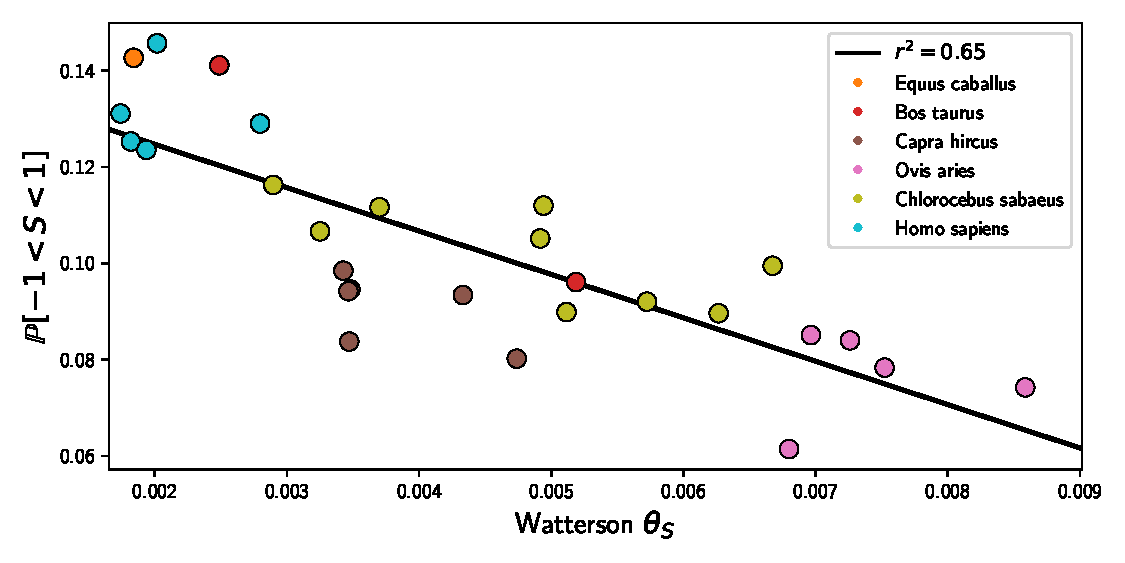
\includegraphics[width=\linewidth, page=1]{../experiments/3bins-mC-masked/regression-MutSel/results.watterson.all_P-Sweak.scatter.pdf}
    \end{minipage}
    \begin{minipage}{0.49\linewidth}
        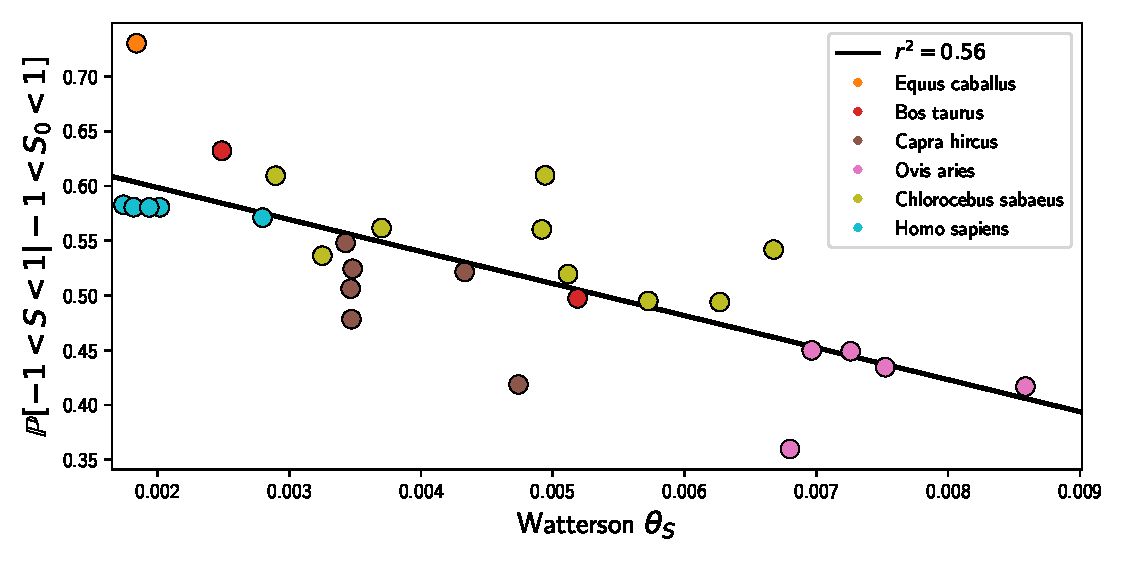
\includegraphics[width=\linewidth, page=1]{../experiments/3bins-mC-masked/regression-MutSel/results.watterson.weak_P-Sweak.scatter.pdf}
    \end{minipage}
    \begin{itemize}
        \item $\ \proba [ \polyNeutral ]$ is the proportion of DFE with a selection coefficient at the population-genetic scale ($\Spop$) between -1 and 1, estimated for the whole genome.
        \item $\ \proba [ \polyNeutral \given \divWeak ]$ is the proportion of DFE with a selection coefficient at the population-genetic scale ($\Spop$) between -1 and 1, estimated of SNPs observed with a selection coefficient at the phylogenetic scale ($\Sphy$) between -1 and 1.
    \end{itemize}

    We confirmed that higher synonymous diversity is typically accompanied by a smaller proportion of neutral mutations.
    This result is specially visible when we restricted the analysis to class of mutations that are supposedly nearly-neutral at the phylogenetic scale ($\divWeak$).
    This result suggests that populations with higher diversity (e.g.~\textit{Bos} or \textit{Ovis}) are more likely to discriminate whether mutations are beneficial or deleterious.
    Alternatively stated, mutations in populations with low diversity (e.g.~\textit{Homo}) are effectively nearly-neutral and behave as would a neutral mutation.
    This result is qualitatively in accordance with the nearly-neutral theory of evolution which argues that mutations are less efficiently selected for in small populations.

    \subsubsection{Proportion of deleterious mutations ($\polyDel$)}\label{subsec:proportion-deleterious-mutations}
    \captionof{figure}{~}
    \begin{minipage}{0.49\linewidth}
        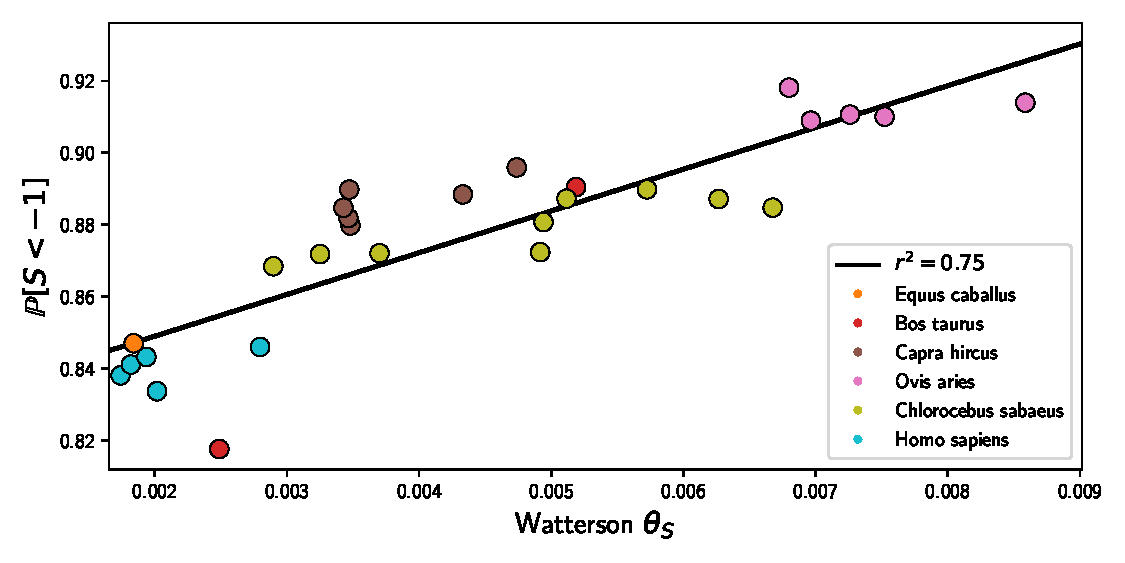
\includegraphics[width=\linewidth, page=1]{../experiments/3bins-mC-masked/regression-MutSel/results.watterson.all_P-Sneg.scatter.pdf}
    \end{minipage}
    \begin{minipage}{0.49\linewidth}
        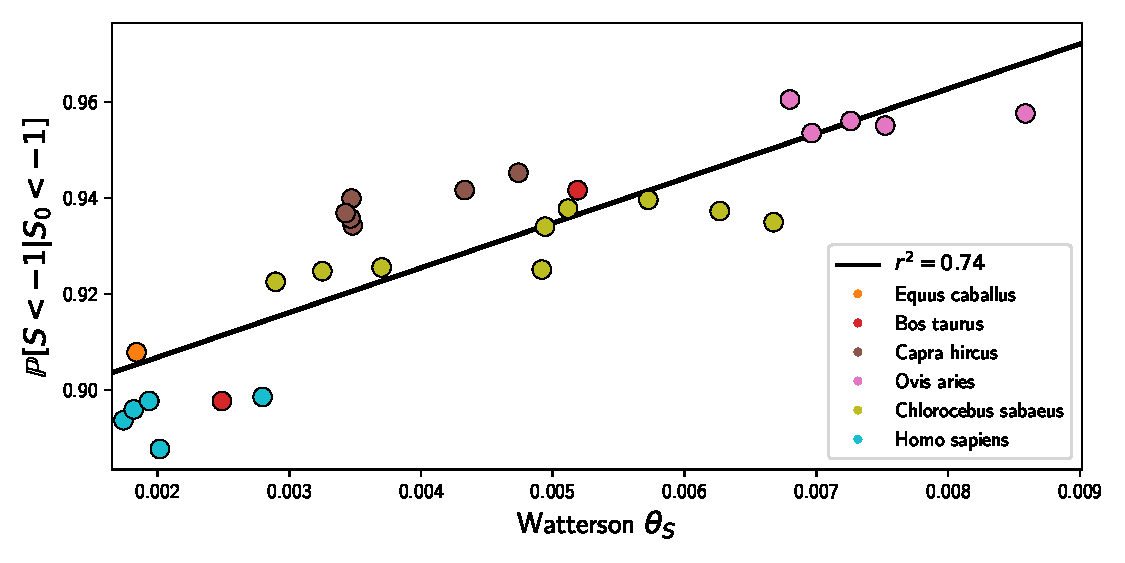
\includegraphics[width=\linewidth, page=1]{../experiments/3bins-mC-masked/regression-MutSel/results.watterson.neg_P-Sneg.scatter.pdf}
    \end{minipage}
    \begin{itemize}
        \item $\ \proba [ \polyDel ]$ is the proportion of DFE with a selection coefficient at the population-genetic scale ($\Spop$) lower than -1, estimated for the whole genome.
        \item $\ \proba [ \polyDel \given \divDel]$ is the proportion of DFE with a selection coefficient at the population-genetic scale ($\Spop$) lower than -1, estimated of SNPs observed with a selection coefficient at the phylogenetic scale ($\Sphy$) lower than -1.
    \end{itemize}

    \subsubsection{Proportion of beneficial mutations ($\polyAdv$)}\label{subsec:proportion-beneficial-mutations}
    \captionof{figure}{~}
    \begin{minipage}{0.49\linewidth}
        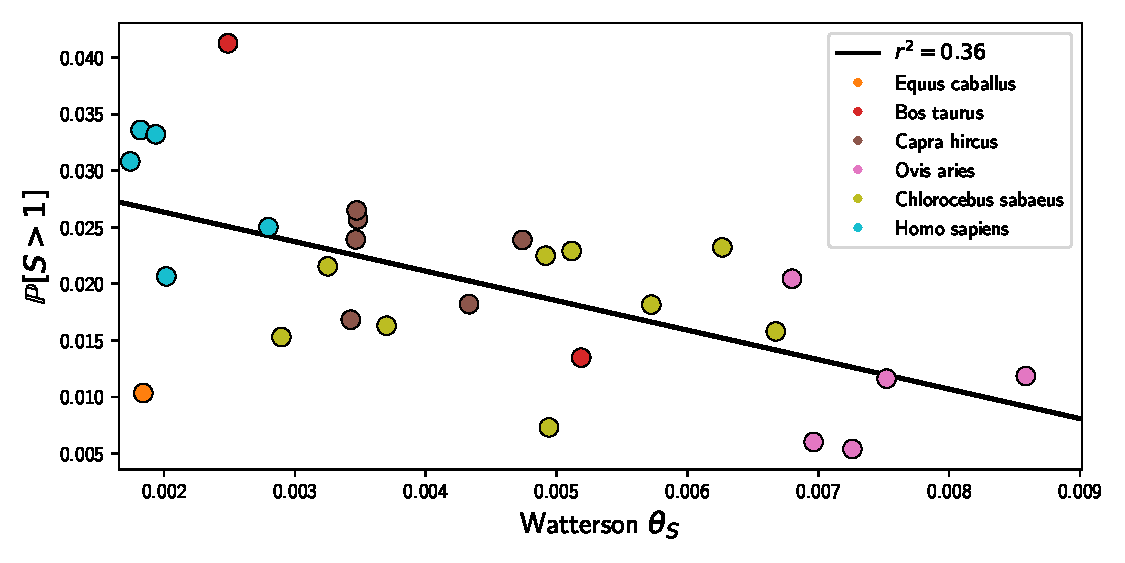
\includegraphics[width=\linewidth, page=1]{../experiments/3bins-mC-masked/regression-MutSel/results.watterson.all_P-Spos.scatter.pdf}
    \end{minipage}
    \begin{minipage}{0.49\linewidth}
        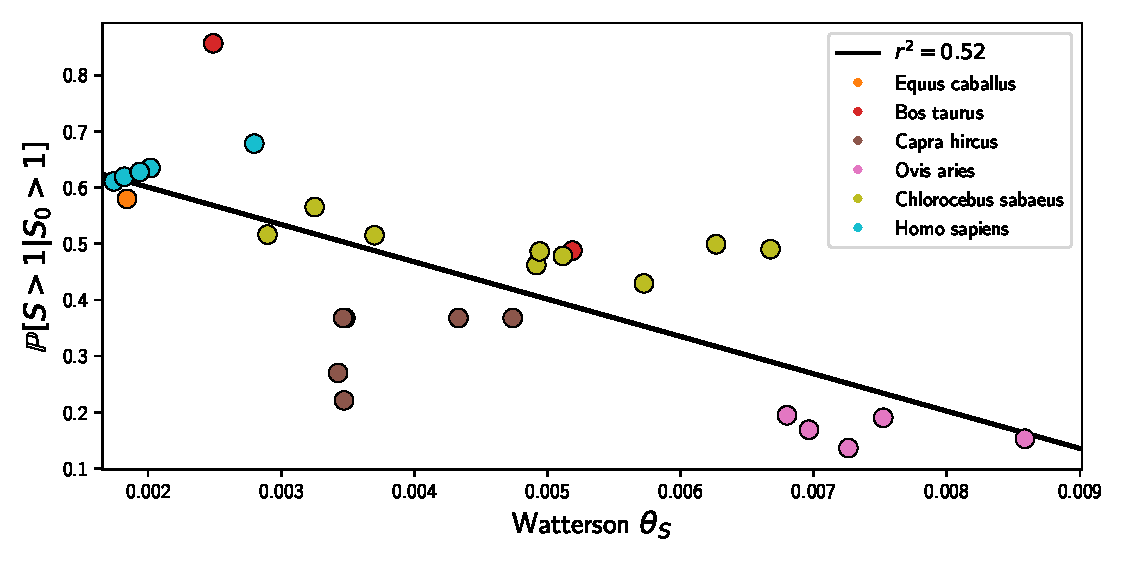
\includegraphics[width=\linewidth, page=1]{../experiments/3bins-mC-masked/regression-MutSel/results.watterson.pos_P-Spos.scatter.pdf}
    \end{minipage}
    \begin{itemize}
        \item $ \proba [ \polyAdv ]$ is the proportion of DFE with a selection coefficient at the population-genetic scale ($\Spop$) greater than 1, estimated for the whole genome.
        \item $\proba [ \polyAdv \given \divAdv] $ is the proportion of DFE with a selection coefficient at the population-genetic scale ($\Spop$) greater than 1, estimated of SNPs observed with a selection coefficient at the phylogenetic scale ($\Sphy$) greater than 1.
    \end{itemize}

    \newpage

    \section{Clinically related terms for non-synonymous mutations}

    \begin{center}
        \captionof{table}{Clinically related terms for $\Sphy < -1$}
        \begin{tabular}{|l|r|r|r|r|r|}
            \toprule
            SNP clinical ontology & $n_{\mathrm{Observed}}$ & $n_{\mathrm{Expected}}$ & Odds ratio & $p_{\mathrm{v}}$ & $p_{\mathrm{v-adjusted}}$ \\
            \midrule
            Benign                & 2969                    & $4043.0$                & $ 0.734$   & $ 1.000$             & $ 1.000~~$                    \\
            Likely benign         & 2994                    & $3399.8$                & $ 0.881$   & $ 0.999$             & $ 1.000~~$                    \\
            Risk factor           & 102                     & $ 118.2$                & $ 0.863$   & $ 0.798$             & $ 1.000~~$                    \\
            Likely pathogenic     & 221                     & $  68.5$                  & $ 3.226$   & $1.7\times 10^{-8}$  & $\bm{6.7\times 10^{-8}{^*}}$  \\
            Pathogenic            & 560                     & $ 193.6$                & $ 2.893$   & $4.2\times 10^{-17}$ & $\bm{2.1\times 10^{-16}{^*}}$ \\
            \bottomrule
        \end{tabular}
    \end{center}
    In humans, non-synonymous SNPs in the test group (deleterious mutations with $\Sphy < -1$) are contrasted to SNPs in the control group (nearly-neutral mutations with $-1 < \Sphy < 1$).
    For each clinical term, a 2x2 contingency tables is built by counting the number of SNPs based on their selection coefficient and their clinical terms (whether they have this specific term or not).
    Fisher's exact tests are then performed for these 2x2 contingency tables.
    $^*$ signify that the$p_{\mathrm{v}}^{\mathrm{adj}}$ corrected for multiple comparison (Holm–Bonferroni correction) is lower than the risk $\alpha=0.05$.
    SNPs predicted with $\Sphy < -1$ are statistically associated to clinical terms such as \textit{Likely Pathogenic} and \textit{Pathogenic}.

    \begin{center}
        \captionof{table}{Clinically related terms for $\Sphy > 1$}
        \begin{tabular}{|l|r|r|r|r|r|}
            \toprule
            SNP clinical ontology & $n_{\mathrm{Observed}}$ & $n_{\mathrm{Expected}}$ & Odds ratio & $p_{\mathrm{v}}$ & $p_{\mathrm{v-adjusted}}$ \\
            \midrule
            Benign                & 319                     & $ 261.7$                & $ 1.219$   & $ 0.002$         & $\bm{ 0.009{^*}}$         \\
            Likely benign         & 263                     & $ 222.7$                & $ 1.181$   & $ 0.012$         & $\bm{ 0.049{^*}}$         \\
            Risk factor           & 5                       & $ 7.847$                & $ 0.637$   & $ 0.879$         & $ 0.879~~$                \\
            Likely pathogenic     & 7                       & $ 4.552$                & $ 1.538$   & $ 0.227$         & $ 0.682~~$                \\
            Pathogenic            & 16                      & $  12.9$                  & $ 1.241$   & $ 0.268$         & $ 0.682~~$                \\
            \bottomrule
        \end{tabular}
    \end{center}
    In humans, non-synonymous SNPs in the test group (beneficial back-mutations with $\Sphy > 1$) are contrasted to SNPs in the control group (nearly-neutral mutations with $-1 < \Sphy < 1$).
    For each clinical term, a 2x2 contingency tables is built by counting the number of SNPs based on their selection coefficient and their clinical terms (whether they have this specific term or not).
    Fisher's exact tests are then performed for these 2x2 contingency tables.
    $^*$ signify that the$p_{\mathrm{v}}^{\mathrm{adj}}$ corrected for multiple comparison (Holm–Bonferroni correction) is lower than the risk $\alpha=0.05$.
    Beneficial back-mutations $\Sphy > 1$ are associated with clinical terms such as \textit{Benign} and \textit{Likely Benign}.

    \newpage

    \section{Distribution of fitness effects}
    \captionof{figure}{~}
    \begin{minipage}{0.49\linewidth}
        \includegraphics[width=\linewidth, page=1]{artworks/2bins.Yeast.experimentalDFE.pdf}
    \end{minipage}
    \begin{minipage}{0.49\linewidth}
        \includegraphics[width=\linewidth, page=1]{artworks/2bins.AFR.histogramDFE.pdf}
    \end{minipage}
    Left panel: distribution of fitness effects experimentally determined in Yeast, data obtained in \textcite{shen_synonymous_2022}.
    Right panel:  distribution of fitness effects ($\Sphy$) as predicted with mutation-selection codon models, from reconstructed ancestral genome in \textit{Homo sapiens}.
    The DFE predicted with mutation-selection codon models has a negative mode, consistently with experimental DFEs, meaning that most mutations are effectively deleterious.

    \newpage

    \section{Mutation-selection models: DFE and SFS for each population}\label{sec:mutation-selection-models:-histograms-and-sfs-for-each-population}
    For each population, the same figure is shown.
    \begin{itemize}
        \item Top-left panel: Distribution of fitness effects ($\Sphy$), predicted for all possible mutations away from the ancestral human genome.
        Mutations are divided into 5 classes of selection: severely deleterious (blue), deleterious (green), weakly deleterious (light green), weakly beneficial (yellow) and beneficial (red, supposedly beneficial back-mutations).
        \item Top-right panel: Histogram of predicted selection coefficients ($\Sphy$) for all observed mutations in a sample of 8 individuals (out of 512 in the original dataset) of African descent.
        If they are less mutations observed than expected, this class is thus undergoing purifying selection.
        \item Bottom-left panel: The site-frequency spectrum (SFS) represents the proportion of mutations (y-axis) with a given number of derived alleles in the population (x-axis).
        SFS are drawn for a random sample of 16 alleles (mean in solid line and standard deviation in filled color) for each class of selection coefficient and for synonymous mutations which are supposedly neutral (black).
        At high frequencies, supposedly severally deleterious mutations are underrepresented.
        \item Bottom-right panel:For each class of selection (and for the set of all non-synonymous mutations), information from the SFS and the expected total mutation rate are combined at the population-genetic scale to estimate the proportion of beneficial mutations $\PpolyAdv$, of nearly-neutral mutations $\PpolyNeutral$ and of deleterious mutations $\PpolyDel$.
    \end{itemize}

    \subsection{All populations}
\begin{center}
    \includegraphics[width=0.95\linewidth, page=1]{../experiments/5bins-polyDFE-mC/results/Theta.MutSel.all.stacked.pdf} \\
    \includegraphics[width=0.95\linewidth, page=1]{../experiments/5bins-polyDFE-mC/results/Theta.MutSel.neg-strong.stacked.pdf} \\
    \includegraphics[width=0.95\linewidth, page=1]{../experiments/5bins-polyDFE-mC/results/Theta.MutSel.neg.stacked.pdf} \\
    \includegraphics[width=0.95\linewidth, page=1]{../experiments/5bins-polyDFE-mC/results/Theta.MutSel.neg-weak.stacked.pdf} \\
    \includegraphics[width=0.95\linewidth, page=1]{../experiments/5bins-polyDFE-mC/results/Theta.MutSel.pos-weak.stacked.pdf} \\
    \includegraphics[width=0.95\linewidth, page=1]{../experiments/5bins-polyDFE-mC/results/Theta.MutSel.pos.stacked.pdf}

\end{center}

\subsection{Bos taurus}

\subsubsection{Iran (IRBT)}

\begin{minipage}{0.49\linewidth}
    \includegraphics[width=\linewidth, page=1]{../data_processed/vcf_annotate_bins5/snps.Bos_taurus.IRBT.MutSel.histogram.pdf}
\end{minipage}
\begin{minipage}{0.49\linewidth}
    \includegraphics[width=\linewidth, page=1]{../experiments/5bins-polyDFE-mC/analysis/Bos_taurus.IRBT.MutSel-sfs.normalize.pdf}
\end{minipage}
\\
\begin{minipage}{0.49\linewidth}
    \includegraphics[width=\linewidth, page=1]{../data_processed/opportunities_bins5/DFE.Bos_taurus.IRBT.MutSel.pdf}
\end{minipage}
\begin{minipage}{0.49\linewidth}
    \includegraphics[width=\linewidth, page=1]{../experiments/5bins-polyDFE-mC/analysis/Bos_taurus.IRBT.MutSel.polyDFE_C.pdf}
\end{minipage}
\\

\subsubsection{Uganda (UGBT)}

\begin{minipage}{0.49\linewidth}
    \includegraphics[width=\linewidth, page=1]{../data_processed/vcf_annotate_bins5/snps.Bos_taurus.UGBT.MutSel.histogram.pdf}
\end{minipage}
\begin{minipage}{0.49\linewidth}
    \includegraphics[width=\linewidth, page=1]{../experiments/5bins-polyDFE-mC/analysis/Bos_taurus.UGBT.MutSel-sfs.normalize.pdf}
\end{minipage}
\\
\begin{minipage}{0.49\linewidth}
    \includegraphics[width=\linewidth, page=1]{../data_processed/opportunities_bins5/DFE.Bos_taurus.UGBT.MutSel.pdf}
\end{minipage}
\begin{minipage}{0.49\linewidth}
    \includegraphics[width=\linewidth, page=1]{../experiments/5bins-polyDFE-mC/analysis/Bos_taurus.UGBT.MutSel.polyDFE_C.pdf}
\end{minipage}
\\

\subsection{Canis familiaris}

\begin{minipage}{0.49\linewidth}
    \includegraphics[width=\linewidth, page=1]{../data_processed/vcf_annotate_bins5/snps.Canis_familiaris.dogs.MutSel.histogram.pdf}
\end{minipage}
\begin{minipage}{0.49\linewidth}
    \includegraphics[width=\linewidth, page=1]{../experiments/5bins-polyDFE-mC/analysis/Canis_familiaris.dogs.MutSel-sfs.normalize.pdf}
\end{minipage}
\\
\begin{minipage}{0.49\linewidth}
    \includegraphics[width=\linewidth, page=1]{../data_processed/opportunities_bins5/DFE.Canis_familiaris.dogs.MutSel.pdf}
\end{minipage}
\begin{minipage}{0.49\linewidth}
    \includegraphics[width=\linewidth, page=1]{../experiments/5bins-polyDFE-mC/analysis/Canis_familiaris.dogs.MutSel.polyDFE_C.pdf}
\end{minipage}
\\

\subsection{Capra}

\subsubsection{Australia (AUCH) - Capra hircus}

\begin{minipage}{0.49\linewidth}
    \includegraphics[width=\linewidth, page=1]{../data_processed/vcf_annotate_bins5/snps.Capra_hircus.AUCH.MutSel.histogram.pdf}
\end{minipage}
\begin{minipage}{0.49\linewidth}
    \includegraphics[width=\linewidth, page=1]{../experiments/5bins-polyDFE-mC/analysis/Capra_hircus.AUCH.MutSel-sfs.normalize.pdf}
\end{minipage}
\\
\begin{minipage}{0.49\linewidth}
    \includegraphics[width=\linewidth, page=1]{../data_processed/opportunities_bins5/DFE.Capra_hircus.AUCH.MutSel.pdf}
\end{minipage}
\begin{minipage}{0.49\linewidth}
    \includegraphics[width=\linewidth, page=1]{../experiments/5bins-polyDFE-mC/analysis/Capra_hircus.AUCH.MutSel.polyDFE_C.pdf}
\end{minipage}
\\

\subsubsection{France (FRCH) - Capra hircus}

\begin{minipage}{0.49\linewidth}
    \includegraphics[width=\linewidth, page=1]{../data_processed/vcf_annotate_bins5/snps.Capra_hircus.FRCH.MutSel.histogram.pdf}
\end{minipage}
\begin{minipage}{0.49\linewidth}
    \includegraphics[width=\linewidth, page=1]{../experiments/5bins-polyDFE-mC/analysis/Capra_hircus.FRCH.MutSel-sfs.normalize.pdf}
\end{minipage}
\\
\begin{minipage}{0.49\linewidth}
    \includegraphics[width=\linewidth, page=1]{../data_processed/opportunities_bins5/DFE.Capra_hircus.FRCH.MutSel.pdf}
\end{minipage}
\begin{minipage}{0.49\linewidth}
    \includegraphics[width=\linewidth, page=1]{../experiments/5bins-polyDFE-mC/analysis/Capra_hircus.FRCH.MutSel.polyDFE_C.pdf}
\end{minipage}
\\

\subsubsection{Iran (IRCA) - Capra aegagrus}

\begin{minipage}{0.49\linewidth}
    \includegraphics[width=\linewidth, page=1]{../data_processed/vcf_annotate_bins5/snps.Capra_hircus.IRCA.MutSel.histogram.pdf}
\end{minipage}
\begin{minipage}{0.49\linewidth}
    \includegraphics[width=\linewidth, page=1]{../experiments/5bins-polyDFE-mC/analysis/Capra_hircus.IRCA.MutSel-sfs.normalize.pdf}
\end{minipage}
\\
\begin{minipage}{0.49\linewidth}
    \includegraphics[width=\linewidth, page=1]{../data_processed/opportunities_bins5/DFE.Capra_hircus.IRCA.MutSel.pdf}
\end{minipage}
\begin{minipage}{0.49\linewidth}
    \includegraphics[width=\linewidth, page=1]{../experiments/5bins-polyDFE-mC/analysis/Capra_hircus.IRCA.MutSel.polyDFE_C.pdf}
\end{minipage}
\\

\subsubsection{Iran (IRCH) - Capra hircus}

\begin{minipage}{0.49\linewidth}
    \includegraphics[width=\linewidth, page=1]{../data_processed/vcf_annotate_bins5/snps.Capra_hircus.IRCH.MutSel.histogram.pdf}
\end{minipage}
\begin{minipage}{0.49\linewidth}
    \includegraphics[width=\linewidth, page=1]{../experiments/5bins-polyDFE-mC/analysis/Capra_hircus.IRCH.MutSel-sfs.normalize.pdf}
\end{minipage}
\\
\begin{minipage}{0.49\linewidth}
    \includegraphics[width=\linewidth, page=1]{../data_processed/opportunities_bins5/DFE.Capra_hircus.IRCH.MutSel.pdf}
\end{minipage}
\begin{minipage}{0.49\linewidth}
    \includegraphics[width=\linewidth, page=1]{../experiments/5bins-polyDFE-mC/analysis/Capra_hircus.IRCH.MutSel.polyDFE_C.pdf}
\end{minipage}
\\

\subsubsection{Italy (ITCH) - Capra hircus}

\begin{minipage}{0.49\linewidth}
    \includegraphics[width=\linewidth, page=1]{../data_processed/vcf_annotate_bins5/snps.Capra_hircus.ITCH.MutSel.histogram.pdf}
\end{minipage}
\begin{minipage}{0.49\linewidth}
    \includegraphics[width=\linewidth, page=1]{../experiments/5bins-polyDFE-mC/analysis/Capra_hircus.ITCH.MutSel-sfs.normalize.pdf}
\end{minipage}
\\
\begin{minipage}{0.49\linewidth}
    \includegraphics[width=\linewidth, page=1]{../data_processed/opportunities_bins5/DFE.Capra_hircus.ITCH.MutSel.pdf}
\end{minipage}
\begin{minipage}{0.49\linewidth}
    \includegraphics[width=\linewidth, page=1]{../experiments/5bins-polyDFE-mC/analysis/Capra_hircus.ITCH.MutSel.polyDFE_C.pdf}
\end{minipage}
\\

\subsubsection{Morocco (MOCH) - Capra hircus}

\begin{minipage}{0.49\linewidth}
    \includegraphics[width=\linewidth, page=1]{../data_processed/vcf_annotate_bins5/snps.Capra_hircus.MOCH.MutSel.histogram.pdf}
\end{minipage}
\begin{minipage}{0.49\linewidth}
    \includegraphics[width=\linewidth, page=1]{../experiments/5bins-polyDFE-mC/analysis/Capra_hircus.MOCH.MutSel-sfs.normalize.pdf}
\end{minipage}
\\
\begin{minipage}{0.49\linewidth}
    \includegraphics[width=\linewidth, page=1]{../data_processed/opportunities_bins5/DFE.Capra_hircus.MOCH.MutSel.pdf}
\end{minipage}
\begin{minipage}{0.49\linewidth}
    \includegraphics[width=\linewidth, page=1]{../experiments/5bins-polyDFE-mC/analysis/Capra_hircus.MOCH.MutSel.polyDFE_C.pdf}
\end{minipage}
\\

\subsection{Chlorocebus sabaeus}

\subsubsection{Barbados}

\begin{minipage}{0.49\linewidth}
    \includegraphics[width=\linewidth, page=1]{../data_processed/vcf_annotate_bins5/snps.Chlorocebus_sabaeus.Barbados.MutSel.histogram.pdf}
\end{minipage}
\begin{minipage}{0.49\linewidth}
    \includegraphics[width=\linewidth, page=1]{../experiments/5bins-polyDFE-mC/analysis/Chlorocebus_sabaeus.Barbados.MutSel-sfs.normalize.pdf}
\end{minipage}
\\
\begin{minipage}{0.49\linewidth}
    \includegraphics[width=\linewidth, page=1]{../data_processed/opportunities_bins5/DFE.Chlorocebus_sabaeus.Barbados.MutSel.pdf}
\end{minipage}
\begin{minipage}{0.49\linewidth}
    \includegraphics[width=\linewidth, page=1]{../experiments/5bins-polyDFE-mC/analysis/Chlorocebus_sabaeus.Barbados.MutSel.polyDFE_C.pdf}
\end{minipage}
\\

\subsubsection{Central African Republic (CAR)}

\begin{minipage}{0.49\linewidth}
    \includegraphics[width=\linewidth, page=1]{../data_processed/vcf_annotate_bins5/snps.Chlorocebus_sabaeus.Central_African_Republic.MutSel.histogram.pdf}
\end{minipage}
\begin{minipage}{0.49\linewidth}
    \includegraphics[width=\linewidth, page=1]{../experiments/5bins-polyDFE-mC/analysis/Chlorocebus_sabaeus.Central_African_Republic.MutSel-sfs.normalize.pdf}
\end{minipage}
\\
\begin{minipage}{0.49\linewidth}
    \includegraphics[width=\linewidth, page=1]{../data_processed/opportunities_bins5/DFE.Chlorocebus_sabaeus.Central_African_Republic.MutSel.pdf}
\end{minipage}
\begin{minipage}{0.49\linewidth}
    \includegraphics[width=\linewidth, page=1]{../experiments/5bins-polyDFE-mC/analysis/Chlorocebus_sabaeus.Central_African_Republic.MutSel.polyDFE_C.pdf}
\end{minipage}
\\

\subsubsection{Ethiopia}

\begin{minipage}{0.49\linewidth}
    \includegraphics[width=\linewidth, page=1]{../data_processed/vcf_annotate_bins5/snps.Chlorocebus_sabaeus.Ethiopia.MutSel.histogram.pdf}
\end{minipage}
\begin{minipage}{0.49\linewidth}
    \includegraphics[width=\linewidth, page=1]{../experiments/5bins-polyDFE-mC/analysis/Chlorocebus_sabaeus.Ethiopia.MutSel-sfs.normalize.pdf}
\end{minipage}
\\
\begin{minipage}{0.49\linewidth}
    \includegraphics[width=\linewidth, page=1]{../data_processed/opportunities_bins5/DFE.Chlorocebus_sabaeus.Ethiopia.MutSel.pdf}
\end{minipage}
\begin{minipage}{0.49\linewidth}
    \includegraphics[width=\linewidth, page=1]{../experiments/5bins-polyDFE-mC/analysis/Chlorocebus_sabaeus.Ethiopia.MutSel.polyDFE_C.pdf}
\end{minipage}
\\

\subsubsection{Gambia}

\begin{minipage}{0.49\linewidth}
    \includegraphics[width=\linewidth, page=1]{../data_processed/vcf_annotate_bins5/snps.Chlorocebus_sabaeus.Gambia.MutSel.histogram.pdf}
\end{minipage}
\begin{minipage}{0.49\linewidth}
    \includegraphics[width=\linewidth, page=1]{../experiments/5bins-polyDFE-mC/analysis/Chlorocebus_sabaeus.Gambia.MutSel-sfs.normalize.pdf}
\end{minipage}
\\
\begin{minipage}{0.49\linewidth}
    \includegraphics[width=\linewidth, page=1]{../data_processed/opportunities_bins5/DFE.Chlorocebus_sabaeus.Gambia.MutSel.pdf}
\end{minipage}
\begin{minipage}{0.49\linewidth}
    \includegraphics[width=\linewidth, page=1]{../experiments/5bins-polyDFE-mC/analysis/Chlorocebus_sabaeus.Gambia.MutSel.polyDFE_C.pdf}
\end{minipage}
\\

\subsubsection{Kenya}

\begin{minipage}{0.49\linewidth}
    \includegraphics[width=\linewidth, page=1]{../data_processed/vcf_annotate_bins5/snps.Chlorocebus_sabaeus.Kenya.MutSel.histogram.pdf}
\end{minipage}
\begin{minipage}{0.49\linewidth}
    \includegraphics[width=\linewidth, page=1]{../experiments/5bins-polyDFE-mC/analysis/Chlorocebus_sabaeus.Kenya.MutSel-sfs.normalize.pdf}
\end{minipage}
\\
\begin{minipage}{0.49\linewidth}
    \includegraphics[width=\linewidth, page=1]{../data_processed/opportunities_bins5/DFE.Chlorocebus_sabaeus.Kenya.MutSel.pdf}
\end{minipage}
\begin{minipage}{0.49\linewidth}
    \includegraphics[width=\linewidth, page=1]{../experiments/5bins-polyDFE-mC/analysis/Chlorocebus_sabaeus.Kenya.MutSel.polyDFE_C.pdf}
\end{minipage}
\\

\subsubsection{Nevis}

\begin{minipage}{0.49\linewidth}
    \includegraphics[width=\linewidth, page=1]{../data_processed/vcf_annotate_bins5/snps.Chlorocebus_sabaeus.Nevis.MutSel.histogram.pdf}
\end{minipage}
\begin{minipage}{0.49\linewidth}
    \includegraphics[width=\linewidth, page=1]{../experiments/5bins-polyDFE-mC/analysis/Chlorocebus_sabaeus.Nevis.MutSel-sfs.normalize.pdf}
\end{minipage}
\\
\begin{minipage}{0.49\linewidth}
    \includegraphics[width=\linewidth, page=1]{../data_processed/opportunities_bins5/DFE.Chlorocebus_sabaeus.Nevis.MutSel.pdf}
\end{minipage}
\begin{minipage}{0.49\linewidth}
    \includegraphics[width=\linewidth, page=1]{../experiments/5bins-polyDFE-mC/analysis/Chlorocebus_sabaeus.Nevis.MutSel.polyDFE_C.pdf}
\end{minipage}
\\

\subsubsection{Saint Kitts (SK)}

\begin{minipage}{0.49\linewidth}
    \includegraphics[width=\linewidth, page=1]{../data_processed/vcf_annotate_bins5/snps.Chlorocebus_sabaeus.Saint_Kitts.MutSel.histogram.pdf}
\end{minipage}
\begin{minipage}{0.49\linewidth}
    \includegraphics[width=\linewidth, page=1]{../experiments/5bins-polyDFE-mC/analysis/Chlorocebus_sabaeus.Saint_Kitts.MutSel-sfs.normalize.pdf}
\end{minipage}
\\
\begin{minipage}{0.49\linewidth}
    \includegraphics[width=\linewidth, page=1]{../data_processed/opportunities_bins5/DFE.Chlorocebus_sabaeus.Saint_Kitts.MutSel.pdf}
\end{minipage}
\begin{minipage}{0.49\linewidth}
    \includegraphics[width=\linewidth, page=1]{../experiments/5bins-polyDFE-mC/analysis/Chlorocebus_sabaeus.Saint_Kitts.MutSel.polyDFE_C.pdf}
\end{minipage}
\\

\subsubsection{South Africa (SA)}

\begin{minipage}{0.49\linewidth}
    \includegraphics[width=\linewidth, page=1]{../data_processed/vcf_annotate_bins5/snps.Chlorocebus_sabaeus.South_Africa.MutSel.histogram.pdf}
\end{minipage}
\begin{minipage}{0.49\linewidth}
    \includegraphics[width=\linewidth, page=1]{../experiments/5bins-polyDFE-mC/analysis/Chlorocebus_sabaeus.South_Africa.MutSel-sfs.normalize.pdf}
\end{minipage}
\\
\begin{minipage}{0.49\linewidth}
    \includegraphics[width=\linewidth, page=1]{../data_processed/opportunities_bins5/DFE.Chlorocebus_sabaeus.South_Africa.MutSel.pdf}
\end{minipage}
\begin{minipage}{0.49\linewidth}
    \includegraphics[width=\linewidth, page=1]{../experiments/5bins-polyDFE-mC/analysis/Chlorocebus_sabaeus.South_Africa.MutSel.polyDFE_C.pdf}
\end{minipage}
\\

\subsubsection{Zambia}

\begin{minipage}{0.49\linewidth}
    \includegraphics[width=\linewidth, page=1]{../data_processed/vcf_annotate_bins5/snps.Chlorocebus_sabaeus.Zambia.MutSel.histogram.pdf}
\end{minipage}
\begin{minipage}{0.49\linewidth}
    \includegraphics[width=\linewidth, page=1]{../experiments/5bins-polyDFE-mC/analysis/Chlorocebus_sabaeus.Zambia.MutSel-sfs.normalize.pdf}
\end{minipage}
\\
\begin{minipage}{0.49\linewidth}
    \includegraphics[width=\linewidth, page=1]{../data_processed/opportunities_bins5/DFE.Chlorocebus_sabaeus.Zambia.MutSel.pdf}
\end{minipage}
\begin{minipage}{0.49\linewidth}
    \includegraphics[width=\linewidth, page=1]{../experiments/5bins-polyDFE-mC/analysis/Chlorocebus_sabaeus.Zambia.MutSel.polyDFE_C.pdf}
\end{minipage}
\\

\subsection{Equus caballus}

\begin{minipage}{0.49\linewidth}
    \includegraphics[width=\linewidth, page=1]{../data_processed/vcf_annotate_bins5/snps.Equus_caballus.up.MutSel.histogram.pdf}
\end{minipage}
\begin{minipage}{0.49\linewidth}
    \includegraphics[width=\linewidth, page=1]{../experiments/5bins-polyDFE-mC/analysis/Equus_caballus.up.MutSel-sfs.normalize.pdf}
\end{minipage}
\\
\begin{minipage}{0.49\linewidth}
    \includegraphics[width=\linewidth, page=1]{../data_processed/opportunities_bins5/DFE.Equus_caballus.up.MutSel.pdf}
\end{minipage}
\begin{minipage}{0.49\linewidth}
    \includegraphics[width=\linewidth, page=1]{../experiments/5bins-polyDFE-mC/analysis/Equus_caballus.up.MutSel.polyDFE_C.pdf}
\end{minipage}
\\

\subsection{Homo sapiens}

\subsubsection{African (AFR)}

\begin{minipage}{0.49\linewidth}
    \includegraphics[width=\linewidth, page=1]{../data_processed/vcf_annotate_bins5/snps.Homo_sapiens.AFR.MutSel.histogram.pdf}
\end{minipage}
\begin{minipage}{0.49\linewidth}
    \includegraphics[width=\linewidth, page=1]{../experiments/5bins-polyDFE-mC/analysis/Homo_sapiens.AFR.MutSel-sfs.normalize.pdf}
\end{minipage}
\\
\begin{minipage}{0.49\linewidth}
    \includegraphics[width=\linewidth, page=1]{../data_processed/opportunities_bins5/DFE.Homo_sapiens.AFR.MutSel.pdf}
\end{minipage}
\begin{minipage}{0.49\linewidth}
    \includegraphics[width=\linewidth, page=1]{../experiments/5bins-polyDFE-mC/analysis/Homo_sapiens.AFR.MutSel.polyDFE_C.pdf}
\end{minipage}
\\

\subsubsection{Ad Mixed American (AMR)}

\begin{minipage}{0.49\linewidth}
    \includegraphics[width=\linewidth, page=1]{../data_processed/vcf_annotate_bins5/snps.Homo_sapiens.AMR.MutSel.histogram.pdf}
\end{minipage}
\begin{minipage}{0.49\linewidth}
    \includegraphics[width=\linewidth, page=1]{../experiments/5bins-polyDFE-mC/analysis/Homo_sapiens.AMR.MutSel-sfs.normalize.pdf}
\end{minipage}
\\
\begin{minipage}{0.49\linewidth}
    \includegraphics[width=\linewidth, page=1]{../data_processed/opportunities_bins5/DFE.Homo_sapiens.AMR.MutSel.pdf}
\end{minipage}
\begin{minipage}{0.49\linewidth}
    \includegraphics[width=\linewidth, page=1]{../experiments/5bins-polyDFE-mC/analysis/Homo_sapiens.AMR.MutSel.polyDFE_C.pdf}
\end{minipage}
\\

\subsubsection{East Asian (EAS)}

\begin{minipage}{0.49\linewidth}
    \includegraphics[width=\linewidth, page=1]{../data_processed/vcf_annotate_bins5/snps.Homo_sapiens.EAS.MutSel.histogram.pdf}
\end{minipage}
\begin{minipage}{0.49\linewidth}
    \includegraphics[width=\linewidth, page=1]{../experiments/5bins-polyDFE-mC/analysis/Homo_sapiens.EAS.MutSel-sfs.normalize.pdf}
\end{minipage}
\\
\begin{minipage}{0.49\linewidth}
    \includegraphics[width=\linewidth, page=1]{../data_processed/opportunities_bins5/DFE.Homo_sapiens.EAS.MutSel.pdf}
\end{minipage}
\begin{minipage}{0.49\linewidth}
    \includegraphics[width=\linewidth, page=1]{../experiments/5bins-polyDFE-mC/analysis/Homo_sapiens.EAS.MutSel.polyDFE_C.pdf}
\end{minipage}
\\

\subsubsection{European (EUR)}

\begin{minipage}{0.49\linewidth}
    \includegraphics[width=\linewidth, page=1]{../data_processed/vcf_annotate_bins5/snps.Homo_sapiens.EUR.MutSel.histogram.pdf}
\end{minipage}
\begin{minipage}{0.49\linewidth}
    \includegraphics[width=\linewidth, page=1]{../experiments/5bins-polyDFE-mC/analysis/Homo_sapiens.EUR.MutSel-sfs.normalize.pdf}
\end{minipage}
\\
\begin{minipage}{0.49\linewidth}
    \includegraphics[width=\linewidth, page=1]{../data_processed/opportunities_bins5/DFE.Homo_sapiens.EUR.MutSel.pdf}
\end{minipage}
\begin{minipage}{0.49\linewidth}
    \includegraphics[width=\linewidth, page=1]{../experiments/5bins-polyDFE-mC/analysis/Homo_sapiens.EUR.MutSel.polyDFE_C.pdf}
\end{minipage}
\\

\subsubsection{South Asian (SAS)}

\begin{minipage}{0.49\linewidth}
    \includegraphics[width=\linewidth, page=1]{../data_processed/vcf_annotate_bins5/snps.Homo_sapiens.SAS.MutSel.histogram.pdf}
\end{minipage}
\begin{minipage}{0.49\linewidth}
    \includegraphics[width=\linewidth, page=1]{../experiments/5bins-polyDFE-mC/analysis/Homo_sapiens.SAS.MutSel-sfs.normalize.pdf}
\end{minipage}
\\
\begin{minipage}{0.49\linewidth}
    \includegraphics[width=\linewidth, page=1]{../data_processed/opportunities_bins5/DFE.Homo_sapiens.SAS.MutSel.pdf}
\end{minipage}
\begin{minipage}{0.49\linewidth}
    \includegraphics[width=\linewidth, page=1]{../experiments/5bins-polyDFE-mC/analysis/Homo_sapiens.SAS.MutSel.polyDFE_C.pdf}
\end{minipage}
\\

\subsection{Ovis}

\subsubsection{Iran (IROA) - Ovis aries}

\begin{minipage}{0.49\linewidth}
    \includegraphics[width=\linewidth, page=1]{../data_processed/vcf_annotate_bins5/snps.Ovis_aries.IROA.MutSel.histogram.pdf}
\end{minipage}
\begin{minipage}{0.49\linewidth}
    \includegraphics[width=\linewidth, page=1]{../experiments/5bins-polyDFE-mC/analysis/Ovis_aries.IROA.MutSel-sfs.normalize.pdf}
\end{minipage}
\\
\begin{minipage}{0.49\linewidth}
    \includegraphics[width=\linewidth, page=1]{../data_processed/opportunities_bins5/DFE.Ovis_aries.IROA.MutSel.pdf}
\end{minipage}
\begin{minipage}{0.49\linewidth}
    \includegraphics[width=\linewidth, page=1]{../experiments/5bins-polyDFE-mC/analysis/Ovis_aries.IROA.MutSel.polyDFE_C.pdf}
\end{minipage}
\\

\subsubsection{Iran (IROO) - Ovis orientalis}

\begin{minipage}{0.49\linewidth}
    \includegraphics[width=\linewidth, page=1]{../data_processed/vcf_annotate_bins5/snps.Ovis_aries.IROO.MutSel.histogram.pdf}
\end{minipage}
\begin{minipage}{0.49\linewidth}
    \includegraphics[width=\linewidth, page=1]{../experiments/5bins-polyDFE-mC/analysis/Ovis_aries.IROO.MutSel-sfs.normalize.pdf}
\end{minipage}
\\
\begin{minipage}{0.49\linewidth}
    \includegraphics[width=\linewidth, page=1]{../data_processed/opportunities_bins5/DFE.Ovis_aries.IROO.MutSel.pdf}
\end{minipage}
\begin{minipage}{0.49\linewidth}
    \includegraphics[width=\linewidth, page=1]{../experiments/5bins-polyDFE-mC/analysis/Ovis_aries.IROO.MutSel.polyDFE_C.pdf}
\end{minipage}
\\

\subsubsection{Iran (IROV) - Ovis vignei}

\begin{minipage}{0.49\linewidth}
    \includegraphics[width=\linewidth, page=1]{../data_processed/vcf_annotate_bins5/snps.Ovis_aries.IROV.MutSel.histogram.pdf}
\end{minipage}
\begin{minipage}{0.49\linewidth}
    \includegraphics[width=\linewidth, page=1]{../experiments/5bins-polyDFE-mC/analysis/Ovis_aries.IROV.MutSel-sfs.normalize.pdf}
\end{minipage}
\\
\begin{minipage}{0.49\linewidth}
    \includegraphics[width=\linewidth, page=1]{../data_processed/opportunities_bins5/DFE.Ovis_aries.IROV.MutSel.pdf}
\end{minipage}
\begin{minipage}{0.49\linewidth}
    \includegraphics[width=\linewidth, page=1]{../experiments/5bins-polyDFE-mC/analysis/Ovis_aries.IROV.MutSel.polyDFE_C.pdf}
\end{minipage}
\\

\subsubsection{Various (ISGC) - Ovis aries}

\begin{minipage}{0.49\linewidth}
    \includegraphics[width=\linewidth, page=1]{../data_processed/vcf_annotate_bins5/snps.Ovis_aries.ISGC.MutSel.histogram.pdf}
\end{minipage}
\begin{minipage}{0.49\linewidth}
    \includegraphics[width=\linewidth, page=1]{../experiments/5bins-polyDFE-mC/analysis/Ovis_aries.ISGC.MutSel-sfs.normalize.pdf}
\end{minipage}
\\
\begin{minipage}{0.49\linewidth}
    \includegraphics[width=\linewidth, page=1]{../data_processed/opportunities_bins5/DFE.Ovis_aries.ISGC.MutSel.pdf}
\end{minipage}
\begin{minipage}{0.49\linewidth}
    \includegraphics[width=\linewidth, page=1]{../experiments/5bins-polyDFE-mC/analysis/Ovis_aries.ISGC.MutSel.polyDFE_C.pdf}
\end{minipage}
\\

\subsubsection{Morocco (MOOA) - Ovis aries}

\begin{minipage}{0.49\linewidth}
    \includegraphics[width=\linewidth, page=1]{../data_processed/vcf_annotate_bins5/snps.Ovis_aries.MOOA.MutSel.histogram.pdf}
\end{minipage}
\begin{minipage}{0.49\linewidth}
    \includegraphics[width=\linewidth, page=1]{../experiments/5bins-polyDFE-mC/analysis/Ovis_aries.MOOA.MutSel-sfs.normalize.pdf}
\end{minipage}
\\
\begin{minipage}{0.49\linewidth}
    \includegraphics[width=\linewidth, page=1]{../data_processed/opportunities_bins5/DFE.Ovis_aries.MOOA.MutSel.pdf}
\end{minipage}
\begin{minipage}{0.49\linewidth}
    \includegraphics[width=\linewidth, page=1]{../experiments/5bins-polyDFE-mC/analysis/Ovis_aries.MOOA.MutSel.polyDFE_C.pdf}
\end{minipage}
\\


    \newpage
    \section{References}
    \printbibliography[heading=none]

\end{document}